\chapter{Suchumfang in MCC\label{chap3:Drittes-Kapitel}}

Aufbauend auf die Vorstellung verschiedener Möglichkeiten für die Umsetzung einer Suchfunktionalität aus \autoref{sec2.1:Unterpunkt-1}, wird in folgendem Kapitel der Suchumfang für die unterschiedlichen Möglichkeiten aufgezeigt.

Als Basis wird sich am Funktionsumfang der zukünftigen MES-Lösung \glqq MCC\grqq{} orientiert. Jener Funktionsumfang wird der bestehenden MES-Lösung \glqq E-MES\grqq{} gleichen und ist derzeit noch in der Entwicklungsphase.

Folgend wird somit nach einer Einführung in den zukünftigen Funktionsumfang von \glqq MCC\grqq{} auch definiert, welche Informationen über die Suchfunktionalität gesucht werden können. Betrachtet werden die Suchfunktionalität \glqq Volltextsuche\grqq{}, \glqq facettierte Suche\grqq{}, \glqq semantische Suche\grqq{} und die Kombination \glqq facettierte Volltextsuche\grqq{}.

\section{Funktionsumfang von MCC\label{sec3.1:Unterunterpunkt-1}}

Bei der Neugestaltung der bestehenden MES-Lösung \glqq E-MES\grqq{} wird neben dem Produktnamen hauptsächlich der architekturelle Aufbau der Software angepasst. Der Funktionsumfang von \glqq MCC\grqq{} wird sich dem jetzigen Funktionsumfang von \glqq E-MES\grqq{} angleichen und ihn in Zukunft zusätzlich erweitern.

Die ersten Planungen für die Aufteilung der Funktionen in \glqq MCC\grqq{} sehen eine Aufteilung in vier unterschiedliche Schichten vor. Niedrigere Schichten sollen dabei nicht von höheren Schichten abhängig sein und können somit ohne höhere Schichten existieren. Folgend werden die vier Funktions-Schichten \glqq MCC Platform\grqq{}, \glqq Core Services - Production\grqq{}, \glqq PCS\grqq{} und \glqq SCADA\grqq{} erläutert und es werden die darin enthaltenen Funktionen betrachtet.

In \autoref{fig:mcc_layer} sind die verschiedenen Schichten abgebildet. Zu erkennen ist, dass die Funktionalitäten in der \glqq MCC Platform\grqq{} - Schicht noch keine Anwendungsfunktionalitäten beinhalten. Enthalten sind in der \glqq MCC Platform\grqq{} Funktionalitäten, welche die Grundfunktionen für den reibungslosen Betrieb einer, auf Microservice basierenden, Architektur ermöglichen. \glqq MCC Platform\grqq{} bildet damit die niedrigste Schicht und kann unabhängig von den darüber liegenden Schichten betrieben werden. Aufbauend auf die Grundfunktionalitäten können verschiedene Anwendungen betrieben werden. Im Umfeld der Firma Enisco sind dies Anwendungen für den Betrieb von Produktionsanlagen. Aber auch Branchen-ferne Anwendungen sind durch die Grundfunktionalitäten der \glqq MCC Platform\grqq{} - Schicht umsetzbar.

Im Umfeld von Produktionsanlagen sind die Funktionalitäten von MCC zusätzlich in die Schichten \glqq Core Services - Production\grqq{}, \glqq PCS\grqq{} und \glqq SCADA\grqq{} unterteilt. In \autoref{fig:mcc_layer} ist dabei zu erkennen, dass die \glqq Core Services - Production\grqq{} - Schicht eine Basisschicht für die \glqq PCS\grqq{} und \glqq SCADA\grqq{} - Schichten darstellt. Enthalten sind Funktionen, welche für mehrere übergeordnete Schichten von Interesse sind.

\begin{figure}[H]
    \centering
    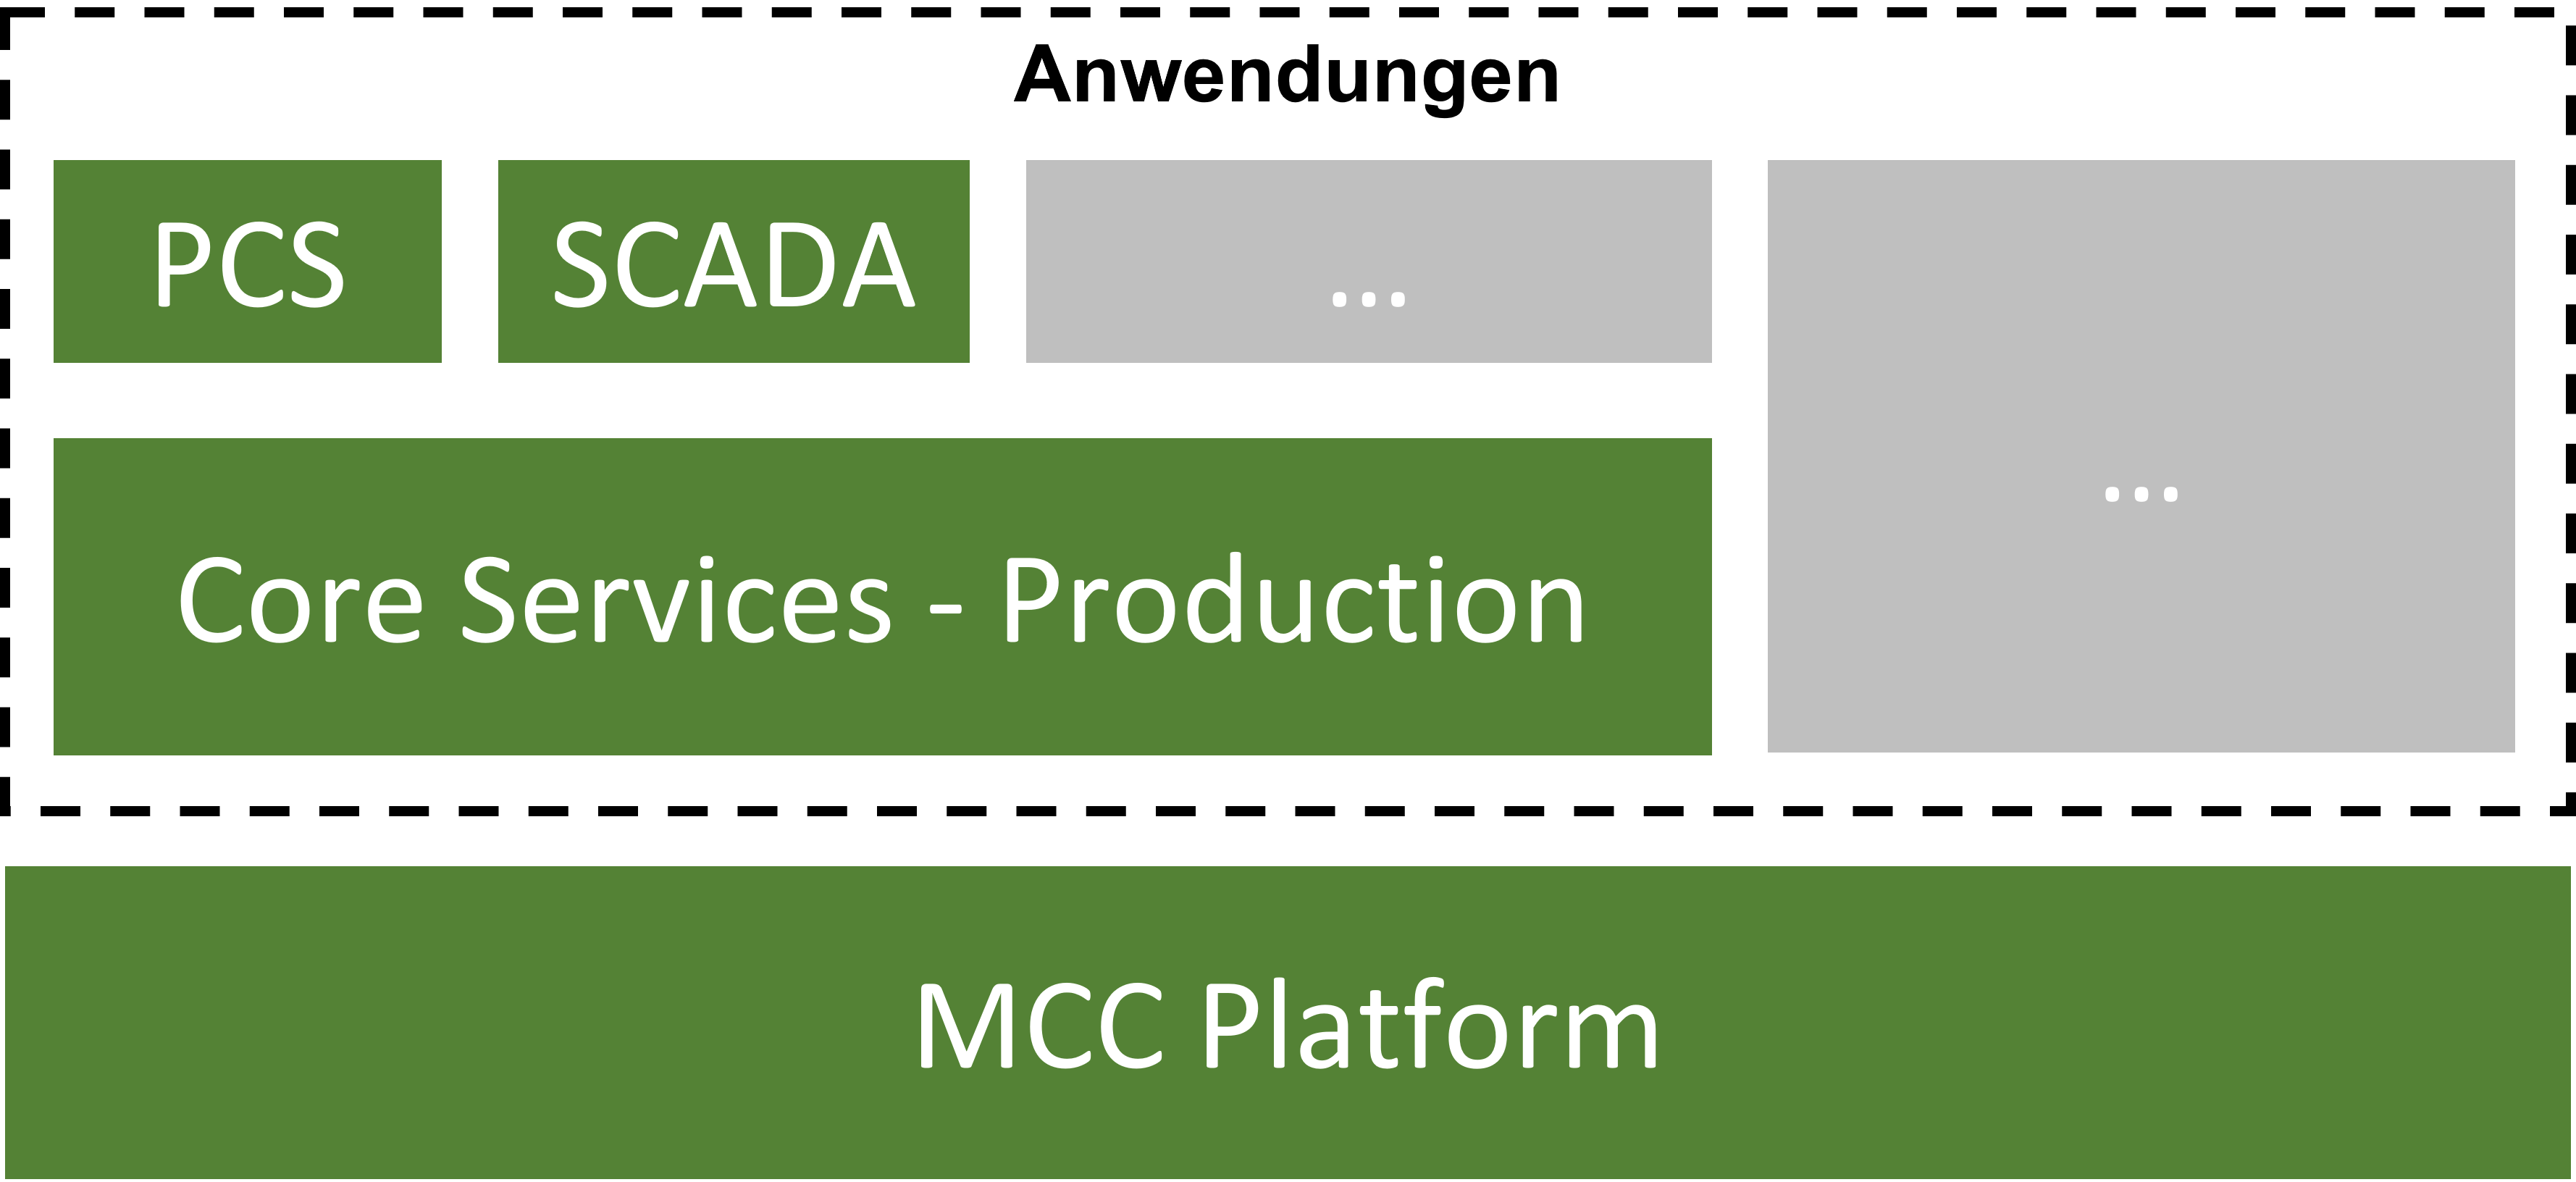
\includegraphics[width=0.7\linewidth]{images/MCC_Layer.png}
    \caption{Übersicht der verschiedenen Layer von MCC}
    \label{fig:mcc_layer}
\end{figure}

Im Folgenden werden die verschiedenen Schichten mit den darin enthaltenen Funktionalitäten abstrahiert erläutert.

\subsection{MCC Platform\label{subsec3.1.1:Unterunterpunkt-1}}

Die Schicht \glqq MCC Platform\grqq{} fungiert als Rahmenschicht für die Anwendungsentwicklung und stellt die Grundfunktionen für die Erstellung und das Betreiben der Anwendungsschichten zur Verfügung.

Zu den Grundfunktionalitäten zählen unteranderem die Themen:

\begin{description}
    \item[Internationalisierung:]\hfill \\
    Um mit einer Software auch eine internationale Kundschaft zu bedienen, ist es erforderlich die Themen Lokalisierung und Internationalisierung zu bedenken. Hierbei geht es darum, mit den länderspezifischen Formaten für Daten und Zahlen und mit unterschiedlichen Zeitzonen umgehen zu können. Auch die Übersetzung der Texte in die jeweilige Sprache wird unter dem Thema Internationalisierung berücksichtigt.
    
    \item[Migrations-API:]\hfill \\
    Aufgrund der späteren Weiterentwicklung der Module kann es bei neuen Versionen dazu kommen, dass sich die Strukturen der Daten in den Datenbanken geändert haben. Bei der Aktualisierung der Module müssen deswegen die bestehenden Daten in den Datenbanken bezüglich der neuen Struktur migriert werden.

    Durch die Umsetzung einer Migrations-API wird nun für jedes Modul eine versionierte Liste mit allen inkrementellen Migrationen abgespeichert. In Kombination mit einem Protokoll, über bereits durchgeführte Migrationen, kann so eine automatische Ausführung der Migration gewährleistet werden.

    \item[Security:]\hfill \\
    Produktionsleitsysteme, wie \glqq E-MES\grqq{}, haben vermehrt einen komplexen Funktionsumfang, welcher bei falscher Bedienung zu hohen Kosten oder Beschädigungen der Anlage führen kann. Aus diesem Grund ist es erforderlich den Zugriff auf bestimmte Aktionen nur für fachkundiges Personal zugänglich zu machen. So können ganze Funktionen für bestimmte Benutzergruppen entweder gesperrt oder durch Weglassen von Bedienelementen angepasst werden.

    Beim Thema \glqq Security\grqq{} geht es demnach um die Authentifizierung und Autorisierung der Benutzer. Neben der Umsetzung von verschiedenen Authentifizierungsmöglichkeiten, müssen den Benutzern die individuellen Rechtepakete zugeordnet werden.

    \item[Streaming Base:]\hfill \\
    Der Austausch von Nachrichten zwischen Microservices wird über Kafka-Topics des Message Brokers \glqq Apache Kafka\grqq{} koordiniert. Der funktionale Ablauf der Nachrichtenweitergabe besteht dabei grundsätzich aus drei Schritten:

    \begin{itemize}
        \item \textbf{Konsumieren} der Nachrichten aus teils mehreren Kafka-Topics
        \item \textbf{Verarbeiten} der Nachrichten (Interaktionen mit den persistenten Speichern oder mit anderen Microservices)
        \item \textbf{Produzieren} der Nachricht an teils mehrere Kafka-Topics
    \end{itemize}

    Unabhängig der späteren Geschäftslogik wird in der \glqq Streaming Base\grqq{} die Kernimplementierung für den Nachrichtentransport implementiert.
    
    \item[Entity Model:]\hfill \\
    In einem Produktionsleitsystem, wie \glqq E-MES\grqq{}, existieren verschiedene Geschäftsentitäten. Die Entitäten mit ihren Attributen unterscheiden sich dabei von Anlage zu Anlage. Deswegen ist es notwendig eine Möglichkeit der Konfiguration bereitzustellen. Durch Import und Export Funktionen soll das Austauschen von Entitätensammlungen vereinheitlicht werden.

    Zusätzlich soll das Entity Model in MCC eine Abstraktion der Datenhaltungsschicht bereistellen, bei welcher verschiedene Abstraktionen für verschiedene Datenbanken zur Verfügung gestellt werden. Über standardisierte API's sollen die jeweiligen Entitäten anschließend abgefragt bzw. bearbeitet werden.

\end{description}

Für den Kontext einer Suchfunktionalität sind die meisten Funktionen nicht relevant, da ein Benutzer mit diesen Funktionen nicht direkt interagiert. Zum Beispiel soll die Funktions- und Arbeitsweise der \glqq Streaming Base\grqq{} dem Benutzer verborgen bleiben.

Geeignet für den Kontext einer Suchfunktionalität sind die Objekte und Informationen aus dem \glqq Security\grqq{} - Modul. Dabei kann zum Beispiel nach den unterschiedlichen Benutzerrollen, den damit verbundenen Rechtepaketen oder diversen Benutzerrechten gesucht werden. So kann durch die Suche nach einem Benutzernamen auch die jeweiligen Rechtepakete gefunden werden und durch die Verwendung eines Sicherheitsaudits, können die Aktivitäten nachverfolgt werden.

% Soll die Online-Dokumentation mit in die Platform?

\subsection{Core Services - Production\label{subsec3.1.2:Unterunterpunkt-2}}

Aufbauend auf den Grundfunktionen der \glqq MCC Platform\grqq{}, welche für den Betrieb einer auf Microservices basierenden Architektur benötigt werden, stellt die \glqq Core Services\grqq{} - Schicht die Grundfunktionen für die eigentliche Anwendung zur Verfügung. Im Umfeld von Produktionsanlagen werden Grundfunktionen für die anwendungsspezifischen Schichten \glqq PCS\grqq{} und \glqq SCADA\grqq{} definiert. Oftmals handelt es sich dabei um Funktionen, welche von mehreren darüber liegenden Schichten verwendet werden.

Im Falle des Funktionsumfangs des Produktionsleitsystems \glqq E-MES\grqq{} handelt es sich in dieser Schicht um Funktionen, welche für die übergeordneten Schichten \glqq PCS\grqq{} und \glqq SCADA\grqq{} von Nutzen sind.

Zu den Funktionen zählen zum Beispiel die folgenden Funktionalitäten:

\begin{description}

    \item[Shift Model:]\hfill \\
    Dem Schichtenmodel sind Funktionalitäten für das Anlegen und Verwalten von Schichten zugeordnet. Hierbei sind die Schichten Bestandteil von vielen weiteren Entitäten. So wird zum Beispiel im SCADA-Bereich angegeben, in welcher Schicht gewisse Sensorwerte aufgezeichnet wurden und zu welcher Schicht Fehler- oder Warnmeldungen erschienen sind. Auch im Bereich der Qualitätskontrolle ist die Angabe der Schicht beim Endtecken von Mängeln von Vorteil, um eine spätere Nachverfolgung zu gewährleisten.

    Zu den Schichten gehört auch ein Schichtlogbuch, in welchem die Benutzer die Möglichkeit haben beliebige Freitexte zu den einzelnen Schichten einzugeben. Durch die Verwendung von Vorlagen haben die Benutzer zusätzlich die Möglichkeit die Kategorie der Freitexte festzulegen. So können auch Schadensberichte oder Qualitätsberichte erstellt und den spezifischen Schichten zugeordnet werden.

    \item[Asset Model:]\hfill \\
    Um auch große Anlagen übersichtlich zu strukturieren und dadurch eine Übersichtlichkeit herzustellen, werden Anlagen üblicherweise in sogenannte \glqq Assets\grqq{} unterteilt. Hierbei kann der Begriff \glqq Asset\grqq{} von den einzelnen Maschinen und Sensoren bis hin zur kompletten Anlage reichen. Eine tiefergehende Erläuterung der \glqq Assets\grqq{} bezüglich dem Einsatz im Umfeld eines Produktionsleitsystems wird in \autoref{subsec3.1.3:Unterunterpunkt-3} \textbf{(\nameref{subsec3.1.3:Unterunterpunkt-3})} augezeigt.

\end{description}

Da die Funktionalitäten des Core-Services Grundlagen für die übergeordneten Schichten \glqq SCADA\grqq{} und \glqq PCS\grqq{} sind, besteht eine hohe Relevanz bezüglich dem Suchkontext einer Suchfunktionalität. Durch Eingabe zum Beispiel einer Asset-Bezeichnung, sollen dem Benutzer alle mit dem Asset verknüpften Objekte und Ereignisse aufgelistet werden.

Bezüglich den Schichten eignen sich vor allem die Freitexte der Schichtlogbücher für den Suchkontext einer Volltextsuche. Hierbei sollen dem Benutzer nach Eingabe einer Suchphrase die relevantesten Schichtlogbücher ausgegeben werden.

\subsection{SCADA\label{subsec3.1.3:Unterunterpunkt-3}}

Damit MCC im Umfeld von Produktionsleitsystemen vertrieben werden kann, sind die Funktionalitäten aus der \glqq SCADA\grqq{}-Schicht notwendig. Die \glqq SCADA\grqq{}-Schicht zählt somit zu den anwendungsspezifischen Schichten.

Bei \gls{scada} geht es um die Überwachung und Steuerung von technischen Prozessen in automatisierten Fertigungen \cite{ColeWangsness.2020}. Dabei werden Daten von Maschinen und Sensoren empfangen und somit deren Zustand überwacht. Durch das Sammeln und Speichern solcher Daten, kann eine eine zeitliche Statistik bezüglich den verschiedenen Maschinen und Sensoren angefertigt werden. Mithilfe solcher Statistiken können durch die frühzeitige Erkennung von Unregelmäßigkeiten Stillstände in der Anlage vermieden werden.

Ein SCADA-System besteht dabei häufig aus einer Kombination aus Software- und Hardware-Elementen \cite{copadata.com.2021}. So beginnt die Datenerfassung auf der Ebene der Maschinen und Sensoren bei den \gls{sps}. Die gesammelten Daten werden anschließend an nächsthöhere Ebenen weitergeleitet. In industriellen Anlagen sind dies oftmals Leitstände, bei welchen die Benutzer die Möglichkeit haben mithilfe von einem \gls{hmi} die Steuerung zu überwachen. Eine \gls{hmi}-Schnittstelle ist ein Bestandteil eines SCADA-Systems und dient zu Visualisierung und Bereitstellung einer Interaktionsmöglichkeit zwischen den Benutzern und dem System. Ein Beispiel für eine Visualisierung ist in \autoref{fig:2D_Visu} abgebildet. Sobald eine Verbindung mit den einzelnen SPSen hergestellt wurde, werden in dieser Ansicht die Echtzeitdaten aus dem jeweiligen Bereich der Anlage angezeigt.

\begin{figure}[H]
    \centering
    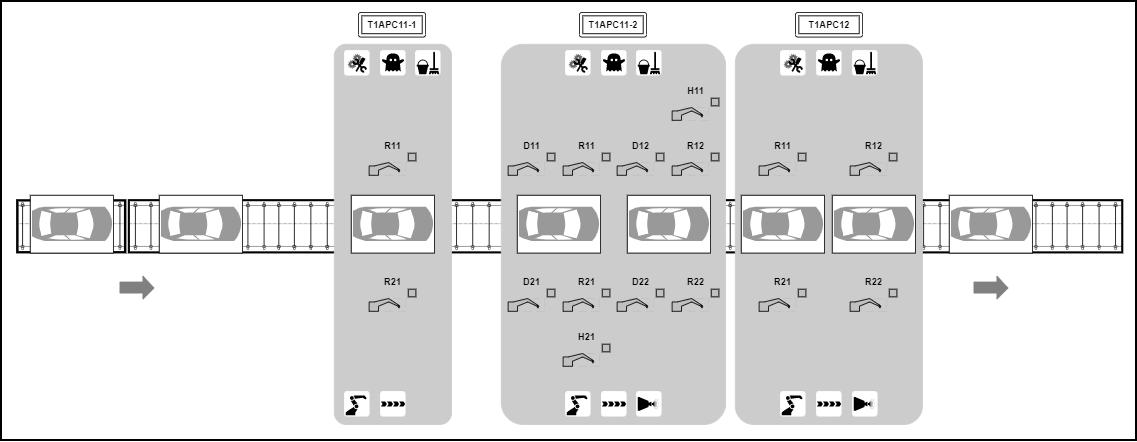
\includegraphics[width=0.8\linewidth]{images/2D_Visu.png}
    \caption{Beispiel für eine HMI in einer SCADA-Umgebung}
    \label{fig:2D_Visu}
\end{figure}

Für den Suchkontext einer Suchfunktionalität im SCADA-Umfeld, gibt es zwei mögliche Sichtweisen auf die Fertigungsanlage:

\begin{description}
    \item[Technische Sicht:]\hfill \\
    Industrielle Fertigungsanlagen durchlaufen während der Lebenzeit mehrere Stadien. Darunter zählt Stadien wie Planung, Entwurf, Realisation, Betrieb, Instandhaltung und Demontage \cite{StefanSchwarzwalder.2019}. Um physische Objekte, innerhalb des Systems und über alle Lebensstadien hinweg eindeutig identifizieren zu können, bedarf es einem einheitlichen Kennzeichnungssystems.

    Als Referenz für solch ein einheitliches Kennzeichnungssystem dient die Norm \glqq EN 81346\grqq{} \cite{StefanSchwarzwalder.2019}. Seit Mai 2005 dient die Norm als einheitliches Kennzeichnungssystem für physikalische Objekte in den Bereichen Elektrotechnik, Maschinenbau und Verfahrenstechnik. Berücksichtigt werden auch Objekte ohne elektrische Relevanz. So werden Objekte, wie Ventile genauso berücksichtigt, wie Schalter und Sensoren. Ziel ist es dadurch das technische System als Gesamtheit zu betrachten \cite{StefanSchwarzwalder.2019}.

    Ein beispielhafter Auszug aus der Norm \glqq EN 81346\grqq{} ist in \autoref{fig:vorzeichen} abgebildet. Gezeigt werden die drei Hauptaspekte \glqq Produktaspekt\grqq, \glqq Funktionsaspekt\grqq und \glqq Ortsaspekt\grqq, welche der Strukturierung der physikalischen Objekte dienen \cite{StefanSchwarzwalder.2019}. So werden den einzelnen Aspekte unterschiedliche Vorzeichen zugeordnet. So können Objekte auf zum Beispiel Schaltplänen eindeutig bezeichnet werden.
    
    \begin{figure}[H]
        \centering
        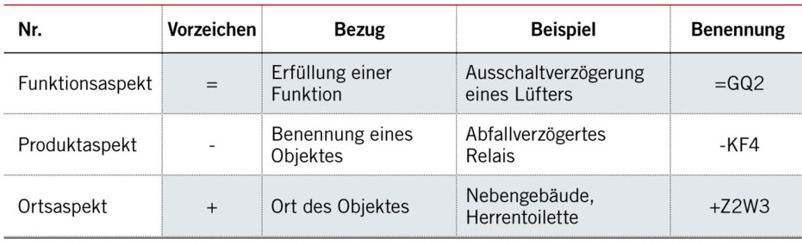
\includegraphics[width=0.8\linewidth]{images/vorzeichen.png}
        \caption{Gliederung der Vorzeichen in EN 81346 \cite{StefanSchwarzwalder.2019}}
        \label{fig:vorzeichen}
    \end{figure}

    % Große Unternehmen mit vielen Fertigungsanlagen verwenden für die Kennzeichnung der Objekte oftmals firmeninterne Kennzeichnungssysteme.

    % Jene Sicht ist vor allem für die Mitarbeiter sinnvoll, welche direkt an den Maschinen arbeiten. Entweder bei der Steuerung der Maschinen oder deren Wartung. Hierbei ist jeder Maschine und jedem Sensor eine eindeutige anlageninterne Codierung zugeteilt.

    % Zum Beispiel => \textbf{T1C041:Visu.P11.1CI1.States.Automatic.Value}

    % Ein Mitarbeiter kann mithilfe der Codierung direkt heraus lesen, in welchem Bereich der Anlage beziehungsweise in welchem Schaltschrank und an welcher SPS die Maschine oder der Sensor angeschlossen ist. So fällt es dem Mitarbeiter leichter Fehler zu finden und die Anlage zu warten.

    \item[Asset Sicht:]\hfill \\
    Neben der technischen Kennzeichnung durch eine einheitliche Kodierung, gibt es zudem die Möglichkeit die Anlage als eine Menge von \glqq Assets\grqq{} zu interpretieren. Hierbei kann der Begriff \glqq Asset\grqq{} von den einzelnen Maschinen und Sensoren bis hin zur kompletten Anlage reichen. Im Gegensatz zur technischen Sichtweise auf die Anlage, können Assets auch gruppiert werden. Es ist zum Beispiel nicht immer notwendig auf der Ebene der einzelnen Maschinen und Sensoren zu interagieren. Die Notwendigkeit den Zustand von zum Beispiel einem hydraulischem Ventil zu erfassen ist im Falle der Wartungsdokumentation gerechtfertigt. Jedoch aus Sicht eines Mitarbeiters, der einen großen Teil der Anlage überwachen und steuern muss, ungeeignet.

    Es ist hilfreich die Assets nach physikalischen Standorten zu gruppieren. So können zum Beispiel verschiedene Antriebsmotoren und Sensoren als \glqq Rollenbahn\grqq{} zusammengefasst werden und dem Mitarbeiter als ein einzelnes Asset dargestellt werden. Die Gruppierung wird dabei solange weitergeführt, bis das Assest \glqq Produktionsanlage\grqq{} erreicht wird. So können mehrere \glqq Rollenbahnen\grqq{} Bestandteile einer \glqq Bearbeitungsstation\grqq{} sein. Und mehrere \glqq Bearbeitungsstationen\grqq{} können zu \glqq Anlagen-Bereichen\grqq{} gruppiert werden. Die dadurch entstandene Hierarchie von Assets kann den kompletten Aufbau der Produktionsanlage widerspiegeln.

    Neben streng hierarchischen Beziehung zwischen Assets können auch logische Beziehungen von Relevanz sein. So ist es möglich, dass mehrere Geräte am selben Bedienfeld angeschlossen sind und darüber eine Beziehungen zueinander haben. Auch eine Gruppierung nach Schaltschränken für die Stromversorgung kann von Relevanz sein. Eine weitere Beziehung zwischen den Assets sind die Materialflüsse, welche beschreiben, wie Produktionseinheiten durch die Produktionsanlage bewegt werden.
    
    % Es gibt demnach verschiedene Arten von Beziehungen zwischen Assets, welche auf physikalischen Verbindungen, wie Zusammensetzung oder Stromversorgung oder auf logischen Verbindungen, wie Materialflüssen beruhen können.
\end{description}

Für den Kontext einer Suchfunktionalität finden sich im SCADA-Umfeld von MCC mehrere Objekte und Informationen, welche relevant für eine Suche sind.

Durch die hierarchische und logische Aufteilung der Produktionsanlage in verschiedene Assets, ist eine Suche nach den expliziten Assets ein relevanter Anwendungsfall und soll durch die Suchfunktionalität in MCC abgedeckt werden. So kann ein Mitarbeiter zum Beispiel nach den Begriffen \glqq Lackierbereich\grqq{}, \glqq Trockenofen\grqq{} oder \glqq Rollenbahn\grqq{} suchen und bekommt eine Auswahl an Funktionen angeboten, welche mit Bezug zu den Assets ausgeführt werden können. Sollte demnach ein Asset mit der Bezeichnung \glqq Rollenbahn\grqq{} im System zu finden sein, sollen dem Mitarbeiter Funktionalitäten, wie die Anzeige von Fehlermeldungen (Alarming) und Auswertung von Prozesswerten (Trending) angeboten werden. Auch die explizite Suche nach bestimmten Schaltschränken oder Pultbereichen kann durch die logische Hierarchie der Assets realisiert werden.

Neben der Verwendung der Assets kann zusätzlich nach dem technischen Kennzeichnungssystem der Maschinen und Sensoren gesucht werden. So kann nach der Eingabe einer Kodierung durch den Benutzer eine Auflistung mit allen relevanten Attributen aufgelistet werden. Darunter zählt zum Beispiel die Zugehörigkeit der Maschine oder des Sensors zu Anlagenbereichen, Pultbereichen oder Schaltschränken.

% Im Grund kann man nach folgenden Objekten suchen:
% \begin{itemize}
%     \item Maschinen/Sensoren (durch deren Codierung)
%     \item Assets
%     \item Pultbereiche
%     \item Schaltschränke
% \end{itemize}

\subsection{PCS\label{subsec3.1.4:Unterunterpunkt-4}}

Neben der \glqq SCADA\grqq{}-Schicht ist die \glqq PCS\grqq{}-Schicht eine weitere anwendungsspezifische Schicht im Funktionsumfang von MCC.

Bei einer \gls{pcs} - Software, geht es um die Aufbereitung der Produktionsaufträge für die jeweilige Anlage. Die eigentlichen Produktionsaufträge, welche in der Produktionsanlage produziert werden sollen, werden von den kundenspezifischen ERP-Systemen eingespeist. Durch die Verwendung von vordefinierten Templates besteht dann die Möglichkeit die Produktionsaufträge automatisiert in verschiedene Jobs zu unterteilen. Für die direkte Anlagensteuerung ist eine weitere Aufteilung in nahezu atomare Arbeitsschritte notwendig. Durch die Einbeziehung von Anlagenressourcen und einer intelligenten Planungssoftware, werden die einzelnen Arbeitsschritte schließlich koordiniert. Exemplarisch ist solch eine Ressourceplanung in \autoref{fig:Ressourcenplanung} abgebildet. Bei der Ressourceplanung wird festgelegt, zu welchem Zeitpunkt ein Bauteil mit seinem passenden Warenträger bei einem bestimmten Arbeitsschritt vorliegt. Mithilfe solch einer Planung wird versucht eine optimale Auslastung der Anlage zu erreichen.

\begin{figure}[H]
    \centering
    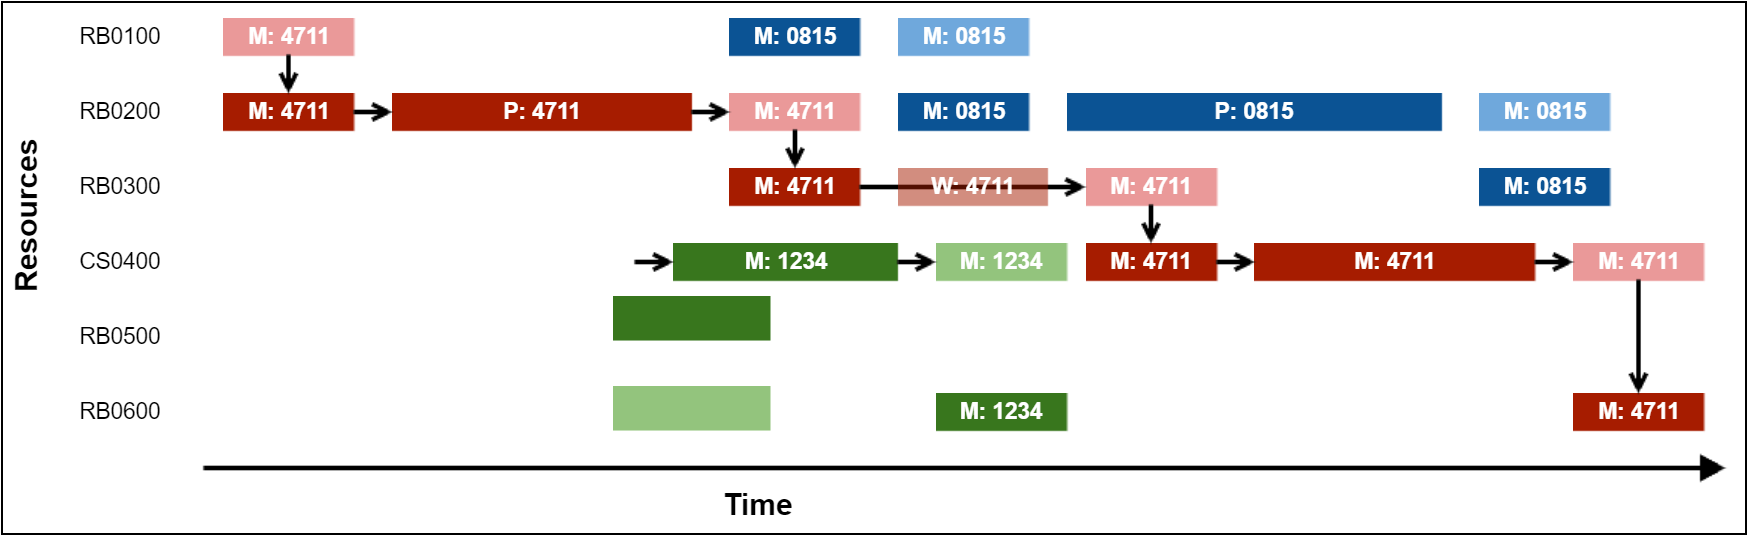
\includegraphics[width=0.9\linewidth]{images/Ressourcenplanung.png}
    \caption{Exemplarische Ressourcenplanung \cite{EniscobyForcamGmbH.2021}\protect\footnotemark}
    \label{fig:Ressourcenplanung}
\end{figure}

\footnotetext{Quelle aus dem Intranet (nicht öffentlich zugänglich) von der Enisco by Forcam GmbH}

Eine weitere Funktionalität von PCS ist das Erstellen einer digitalen Lebenlaufakte für die jeweiligen Produktionsaufträge. Eine Lebenslaufakte ist im Umfeld der digitalen Vernetzung ein Werkzeug zur lückenlosen Dokumentation des Produktlebenszyklus eines industriellen Produktes \cite{MaximilianAusterjost.2021}. Innerhalb einer solchen Akte werden alle anlagenbezogenen Informationen gesammelt und aktuell gehalten. Sie dient als Basis für industrielle Kollaborationen zwischen Anlagenherstellern und IT- und Servicedienstleistern und ist durch die Vielseitigkeit und Anpassungsfähigkeit in den unterschiedlichsten Produktlebenszyklen einsetzbar \cite{MaximilianAusterjost.2021}. Für die Standardisierung einer solchen Lebenslaufakte ist im September 2018 die Norm \glqq EN 77005-1\grqq{} veröffentlicht worden. Innerhalb von MCC wird die Lebenlaufakte sowohl durch die Funktionalitäten der PCS-Schicht, als auch durch die Funktionalitäten der SCADA-Schicht aktuell gehalten. So können neben allgemeinen Informationen zum Produkt auch Werte gespeichert werden, welche bei den einzelnen Arbeitsschritten entstanden sind. So ist eine nachträgliche Auswertung der einzelnen Arbeitsschritte bezüglich dem jeweiligen Produkt möglich.

Für den Kontext einer Suchfunktionalität in MCC sind die Informationen aus den einzelnen Lebenlaufakten von hoher Relevanz. Abhängig von der späteren, tatsächlichen Umsetzung wird jedem Produktionsauftrag und somit jeder Lebenlaufakte eine eindeutige Identifikationsnummer zugeordnet. Mithilfe einer solchen Identifikationsnummer soll es für den Benutzer von MCC möglich sein, unteranderem den Status des Produktionsauftrags und eine Auflistung von noch ausstehenden Arbeitsschritten zu erhalten.

Neben gezielten Informationen zu einzelnen Produkten und den dazugehörigen digitalen Lebenslaufakten sind unteranderem auch Informationen bezüglich den einzelnen Jobs und deren Arbeitsschritte von Relevanz. Hierfür besitzen die einzelnen Prozesse wiederum eine eindeutige Identifikationsnummer. Relevant ist zudem eine gezielte Suche nach den Ressourcen der Produktionsanlage. So kann ein Benutzer eine Identifikationsnummer eines Warenträgers eingeben und erhält alle relevanten Informationen bezüglich dem Warenträger angezeigt.

% Im Grund kann man nach folgenden Objekten suchen:
% \begin{itemize}
%     \item Bauteile
%     \item Aufträge
%     \item Warenträger
%     \item Maschinen
%     \item Arbeitsschritte
% \end{itemize}

\section{Umfang einer Volltextsuche\label{sec3.2:Unterunterpunkt-2}}

Text

\section{Umfang einer facettierten Suche\label{sec3.3:Unterpunkt-3}}

Text

\section{Umfang einer semantischen Suche\label{sec3.4:Unterpunkt-4}}

Text